% !TEX root = ../../main.tex


\begin{figure}[tb]
{\small\texthv{\textbf{\,(a) True IBD}}} \\
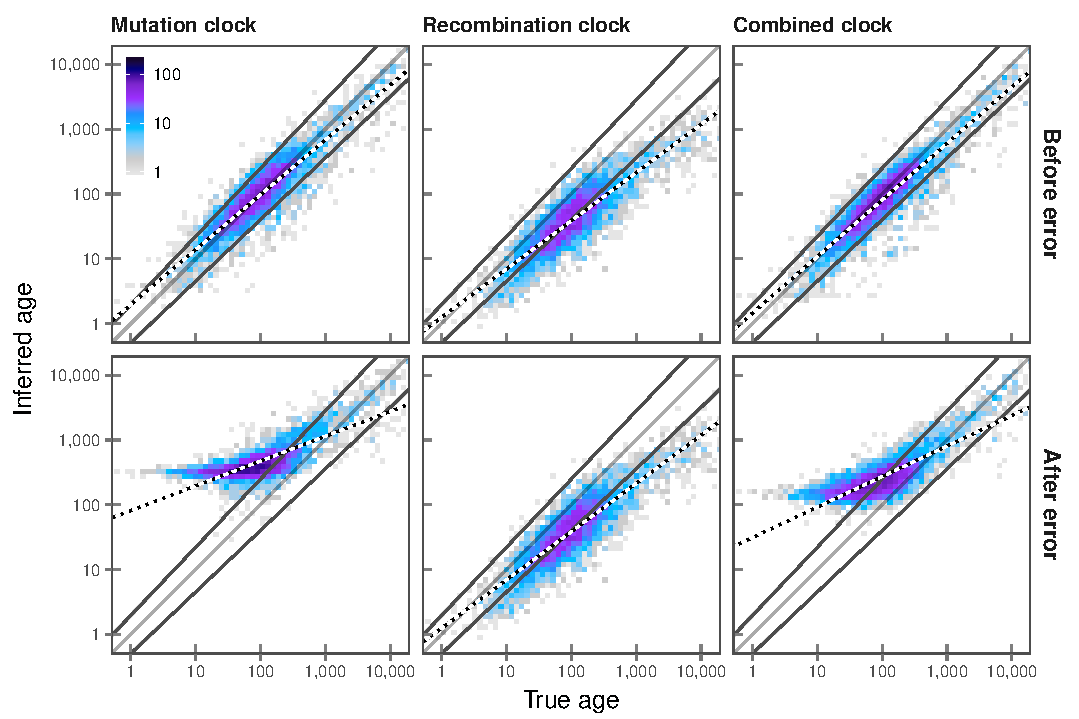
\includegraphics[width=\textwidth]{./img/ch5/generror_scat_tru}
\Caption{Density distribution of allele age before and after the inclusion of genotype error in simulated data}
{Allele age estimation was conducted on data in which empirical distributions of genotype error were simulated.
The effects on the estimation process \emph{before} and \emph{after} error are compared (\emph{top} and \emph{bottom}, respectively).
The dividing line is fixed at the true age ($t_m$), around which the lines \emph{below} and \emph{above} correspond to the regression trend lines of the times of coalescent events delimiting the branch on which focal mutations sit; \ie $t_c$ and $t_d$, respectively.
The \emph{black-white} line indicates the regression trend of the inferred age ($\hat{t}$).
This panel (\textbf{a}) compares the distributions of true and inferred ages, which were estimated on basis of the true IBD structure of the sample as determined from simulation records.
The other panels show estimation results based on the different IBD detection methods;
\gls{fgt} on both true and phased haplotypes (\textbf{b}, \textbf{c}; \pref{fig:generror_scat_fgt}),
\gls{dgt} (\textbf{d}; \pref{fig:generror_scat_dgt}),
and the \gls{hmm}-based approach (\textbf{e}; \pref{fig:generror_scat_hmm}).
Each analysis was conducted on the same set of retained \n{5015} target variants at allele frequency ${\leq 0.5\%}$ in simulated data of ${N=\num{2500}}$ diploid individuals.}
{fig:generror_scat_tru}
\end{figure}
